%# -*- coding: utf-8-unix -*-
\chapter{单体船的窄V字形尾迹}
\label{chap:monohull}

本章考虑在无限深广的静水中匀速直线航行的单体船的窄V字形尾迹。
船体周围的流场以分布在船体表面的点源产生的流场表示,而不是简化为位于船首区域
的一个点源和位于船尾区域的一个点汇。

\section{主要兴波角的确定}
\label{sec:psimaxcalc}

由第\ref{chap:fsG}章的结果可知,只考虑速度势的波浪成分可将船后的波浪势
$\tilde{\phi}^W$写成如下Fourier-Kochin表达式
\begin{equation}
  \tilde{\phi}^W(\tilde{\mathbf{x}})=\frac{F^2}{\pi}\mathrm{Im}
  \int_{-\infty}^{\infty}
  A(q)\tilde{E}(q,\tilde{\mathbf{x}})\,\mathrm{d}q
  \label{eq:fkrepresent}
\end{equation}
其中基波$\tilde{E}(q,\tilde{\mathbf{x}})$由\eqref{eq:Etilde}给出,
波幅$A(q)$由\eqref{eq:Asymmetry}给出。这里已经忽略式\eqref{eq:phiW}中的
短波过滤函数$\tilde{\Lambda}(q,\tilde{\mathbf{x}})$,并将积分上下限由
$\pm q_{\infty}$改为$\pm\infty$。
同样处理式\eqref{eq:fsheight}可得自由面升高
\begin{equation}
  z(\tilde{x},\tilde{y})=\frac{F^2}{\pi}\mathrm{Re}\int_{-\infty}^{\infty}
  \sqrt{1+q^2}A(q)\mathrm{e}^{\mathrm{i}\sqrt{1+q^2}(\tilde{x}+q\tilde{y})/F^2}
  \,\mathrm{d}q
  \label{eq:freesurfelev}
\end{equation}

式\eqref{eq:freesurfelev}可以改写成下式
\begin{equation}
  \frac{Zg}{V^2}=\frac{1}{\pi}\mathrm{Re}\int_{-\infty}^{\infty}
  \sqrt{1+q^2}A\mathrm{e}^{\mathrm{i}h\varphi}\,\mathrm{d}q
  \label{eq:ZgV2}
\end{equation}
这里$h$是以速度无因次化的距离
\begin{eqnarray}
  && h\equiv Hg/V^2\equiv \sqrt{\xi^2+\eta^2}\label{eq:h}\\
  && (\xi,\eta)\equiv (\tilde{x},\tilde{y})/F^2\equiv(\tilde{X},\tilde{Y})g/V^2
  \label{eq:xieta}
\end{eqnarray}
$A$由式\eqref{eq:Asymmetry}定义。相位函数$\varphi$和它的一阶导数
$\varphi'\equiv\mathrm{d}\varphi/\mathrm{d}q$、二阶导数$\varphi''\equiv\mathrm{d}^2\varphi/\mathrm{d}q^2$由式\eqref{eq:faz}定义。在远场$1\ll h$,积分\eqref{eq:ZgV2}
可由第\ref{chap:shipwav}章介绍的驻相法得到解析近似
\begin{eqnarray}
  &&\frac{Zg}{V^2}\approx\sqrt{\frac{2/\pi}{h}}\mathrm{Im}(e^D+e^T)\quad\text{其中}
  \label{eq:ZgV2stat}\\
  &&e^D\equiv A^D\sqrt{\frac{1+(q^D)^2}{\varphi''_D}}\mathrm{e}^{\mathrm{i}h\varphi^D+\pi/4}\label{eq:eD}\\
  &&e^T\equiv A^T\sqrt{\frac{1+(q^T)^2}{-\varphi''_T}}\mathrm{e}^{\mathrm{i}h\varphi^T-\pi/4}\label{eq:eT}
\end{eqnarray}
这里$q^D$和$q^T$由式\eqref{eq:qTD}定义,$A^D$和$A^T$是波幅函数$A$在
$q=q^D$和$q=q^T$处的值。渐近近似\eqref{eq:ZgV2stat}在Kelvin臂附近无效,
因为在Kelvin臂二阶导数$\varphi''_D$和$\varphi''_T$为零,正如第\ref{chap:shipwav}
章所述和众所周知的。此后忽略远场驻相法近似\eqref{eq:ZgV2stat}中的横波$e^T$,
因为在高Froude数情况下,除非在Kelvin臂$\psi=\pm\psi^K$附近,散波占支配地位。
而正如前面指出的,主要兴波角$\psi_{\max}$显著小于Kelvin角$\psi^K$,
因此这种简化是合理的。在Kelvin臂附近时,横波的重要性增加,更准确的分析需要考虑横波。

图\ref{fig:amplfunc}描画了由型宽$b=0.15$型深$d=0.05$的简单船体
\begin{equation}
  y=\pm\frac{b}{2}(1-16x^4)\left(1-\frac{z^2}{d^2}\right)
  \label{eq:simphull}
\end{equation}
在六个Froude数$F=$0.65,0.7,0.9,1.1,1.3和1.5时
产生的散波的波幅函数$\zeta^D\equiv\sqrt{2/\pi}F^2|e^D|$,即
\begin{equation}
  \zeta^D\equiv\sqrt{2/\pi}F^2|A^D|\sqrt{[1+(q^D)^2]/\varphi''_D}
  \label{eq:zetaD}
\end{equation}
%
\begin{figure}[htp]
  \centering
  \captionstyle{\centering}
  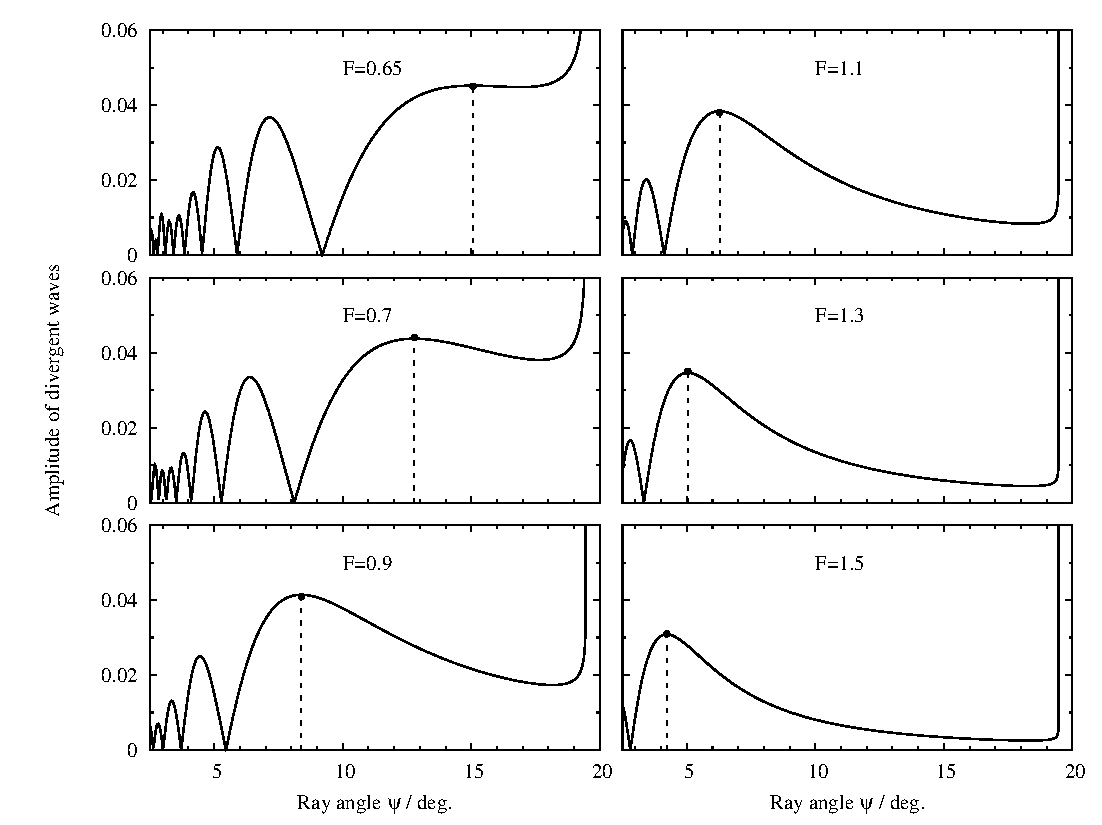
\includegraphics[width=0.8\textwidth]{chap5/amplfunc.pdf}
  \bicaption[fig:amplfunc]{单体船散波的波幅函数}
  {船体\eqref{eq:simphull}在$0.65\le F\le 1.5$范围内六个Froude数情况下产生的散波的
  波幅函数$\zeta^D$,由式?定义,通过Hogner近似计算}{Fig}
  {Amplitude $\zeta^D$ of the divergent waves, defined by \eqref{eq:zetaD}, 
  created by the hull ? and predicted by the Hogner approximation, 
  for $2^\circ30'\le\psi<19^\circ28'$ and six Froude numbers $F$ within the range 
$0.65 \le F \le 1.5$}
\end{figure}

最大波高的波浪所在的射线角$\psi=\psi_{\max}$由波幅函数\eqref{eq:zetaD}
的最高峰确定。此最高峰也是最靠近Kelvin臂的`第一峰',在图\ref{fig:amplfunc}
由一个点和一根竖虚线表示。正如已经指出的,二阶导数$\varphi''_D$在Kelvin臂
$\psi\approx19^\circ28'$为零,此时函数\eqref{eq:zetaD}是无界的。
图\ref{fig:amplfunc}表明通过波幅函数最高峰的位置确定的主要兴波角
$\psi_{\max}$不受函数\eqref{eq:zetaD}在Kelvin臂的弱奇异性的明显影响,
除非可能对$F=0.65$。图\ref{fig:amplfunc}还表明$F\ge0.9$时第一峰锐利,
并显著高于所有其他峰,但在$F\le0.7$时第一峰较宽,并且高出其他峰不多。

\section{数值计算}
\label{sec:numcomput}

现在考虑由七艘船产生的散波的波幅函数\eqref{eq:zetaD}。其中三艘船定义为
\begin{equation}
  y=\pm\frac{b}{2}[1-(2x)^{2n}]\left(1-\frac{z^2}{d^2}\right)
  \label{eq:sevenhull}
\end{equation}
其中$(b,d)=(0.15,0.05)$,$n=1$,2,3。与$n=1$,2,3对应的水线进流角$2\alpha$
约为$33^\circ$,$62^\circ$,$84^\circ$,这三艘船因此分别被称作``锐船'',``中等船'',
和``钝船''。其余四艘船也由式\eqref{eq:sevenhull}定义,其中$n=2$,型宽
$b$和吃水$d$选择为
\begin{equation}
  (b,d)=(0.1,0.1),(0.15,0.075),(0.2,0.05),(0.25,0.025)
  \label{eq:bd4hull}
\end{equation}
这四艘船的型宽船长比和吃水船长比在广阔的范围内$0.1\le b\le0.25$
和$0.025\le d\le0.1$变化,对应的宽度吃水比为1,2,4和10。四艘船的水线进流角$2\alpha$
为:当$b=0.1$时约为$44^\circ$,当$b=0.15$时约为$62^\circ$,当$b=0.2$时约为
$77^\circ$,当$b=0.25$时约为$90^\circ$。计算中考虑的七艘船的型宽船长比$B/L$,
吃水船长比$D/L$,宽度吃水比$B/D$和水线进流角$2\alpha$列于表\ref{tab:7hull}中。
表\ref{tab:7hull}表明七艘船对应的主要船体形状参数在广阔的范围内变化
  \begin{equation}
    \label{eq:shaparam}
  \left.
  \begin{array}{l}
  0.1\le\frac{B}{L}\le0.25,\quad 0.025\le\frac{D}{L}\le 0.1,\\
  1\le\frac{B}{D}\le10,\quad 33^\circ\le2\alpha\le90^\circ
  \end{array}
  \right.
  \end{equation}
\begin{table}
  \centering
  \begin{minipage}[b]{0.6\textwidth}
    \captionstyle{\centering}
  \bicaption[tab:7hull]{七艘单体船的主要船体形状参数}
  {计算中考虑的七艘船的主要船体形状参数}{Table}
  {Main hull-shape parameters associated with the seven hulls considered in the
  computations}
\end{minipage}
  \begin{tabular*}{0.8\textwidth}{@{\extracolsep{\fill}}llrll@{}} \toprule
    $B/L$ & $D/L$ & $B/D$ & $n$ & $2\alpha$ \\ \midrule
    0.15 & 0.05 & 3 & 1 & $33^\circ24'$ \\
    0.15 & 0.05 & 3 & 2 & $61^\circ55'$ \\
    0.15 & 0.05 & 3 & 3 & $83^\circ59'$ \\
    0.1  & 0.1  & 1 & 2 & $43^\circ36'$ \\
    0.15 & 0.075& 2 & 2 & $61^\circ55'$ \\
    0.2  & 0.05 & 4 & 2 & $77^\circ19'$ \\
    0.25 & 0.025&10 & 2 & $90^\circ$ \\ \bottomrule
  \end{tabular*}
\end{table}

图\ref{fig:psimaxmonohull}展示了七艘船在十个Froude数$F\approx0.65$和
$F=0.7$,0.8,$\cdots$,1.5时的主要兴波角$\psi_{\max}$,
由波幅函数\eqref{eq:zetaD}中第一峰的位置确定。
图\ref{fig:psimaxmonohull}表明,船体形状对主要兴波角$\psi_{\max}$的影响不大。
%
\begin{figure}[htp]
  \centering
  \captionstyle{\centering}
  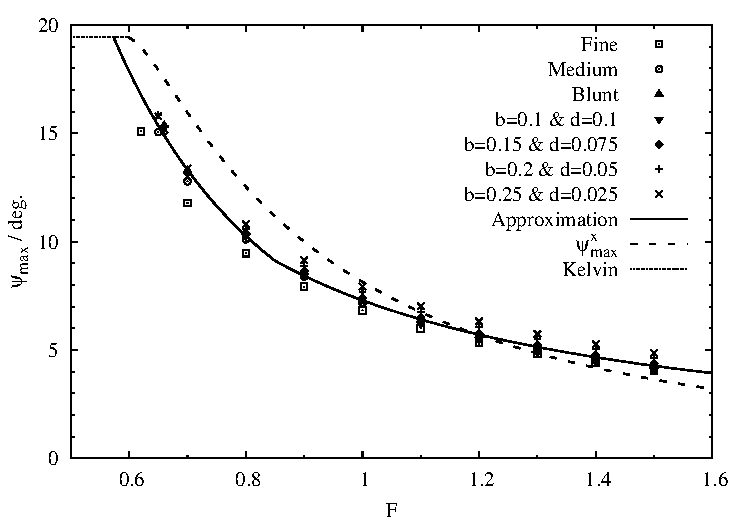
\includegraphics[width=0.8\textwidth]{chap5/psi_max.pdf}
  \bicaption[fig:psimaxmonohull]{单体船的主要兴波角}
  {七艘船在Froude数范围$0.6<F\le1.5$的主要兴波角$\psi_{\max}$,
  由波幅函数\eqref{eq:zetaD}中第一峰的位置确定}{Fig}
  {Apparent wake angle $\psi_{\max}$, determined numerically from the first peak
  of the amplitude function \eqref{eq:zetaD} computed via the Hogner approximation,
for seven hulls and ten Froude numbers within the range $0.6<F<1.5$}
\end{figure}

两点兴波模型中,基于首尾散波系的相干干涉预报的单体船的主要兴波角的表达式
\eqref{eq:psixmax}中$\ell$代表实效船首和实效船尾的实效间距,近似取$\ell=0.9$。
现在通过数值确定的主要兴波角$\psi_{\max}$可以确定实效间距$\ell_e$的大小,即
\begin{eqnarray}
  \ell_e=6.28F^2\tan\psi_{\max}
  \label{eq:elle}
\end{eqnarray}
数值确定的七艘船体在十个Froude数情况下的$\ell_e$的值在图\ref{fig:elleff}中展示。
图\ref{fig:elleff}表明通过式\eqref{eq:elle}得出的实效间距$\ell_e$受船体形状变化
的影响显著,而图\ref{fig:psimaxmonohull}表明主要兴波角$\psi_{\max}$受船体形状
变化的影响很弱,如上所述。因此通过对图\ref{fig:elleff}中$\ell_e$的数值结果进行
粗略的拟合,就足以得到主要兴波角$\psi_{\max}$的实用近似。这里使用
\begin{subequations}\label{eq:ellfit}
\begin{eqnarray}
  \ell_e\approx0.725\quad\text{当}F\le0.85 \label{eq:ell-a}\\
  \ell_e\approx0.3+0.5F\quad\text{当}F\ge0.85 \label{eq:ell-b}
\end{eqnarray}
\end{subequations}
来拟合$\ell_e$. 图\ref{fig:elleff}表明如果拟合中考虑主要的船体形状参数---
特别是型宽船长比---对实效间距$\ell_e$的影响可使$\psi_{\max}$的拟合更加精确。
然而如上所述,船体形状的变化对$\psi_{\max}$的影响很弱,因此$\ell_e$拟合
精度的提高可能对提高$\psi_{\max}$近似精度的作用不大。因此从这个角度看,
用式\eqref{eq:ell-a}和\eqref{eq:ell-b}来拟合$\ell_e$是足够精确的。
%
\begin{figure}[htp]
  \centering
  \captionstyle{\centering}
  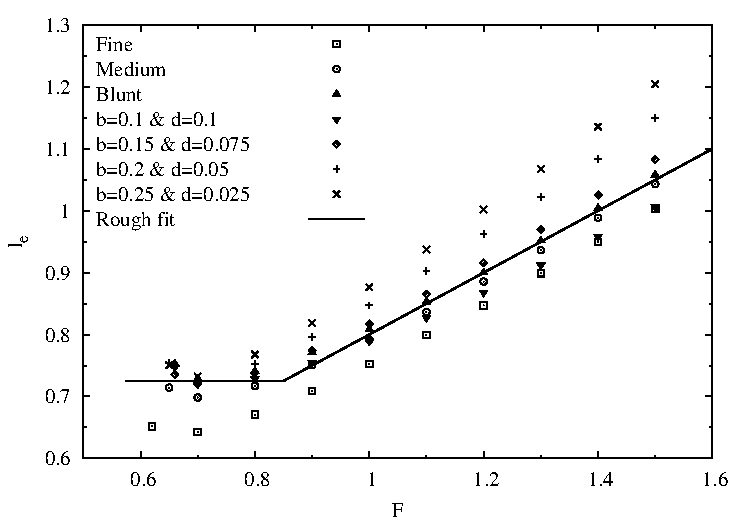
\includegraphics[width=0.8\textwidth]{chap5/l_e.pdf}
  \bicaption[fig:elleff]{实效间距$\ell_e$}
  {式\eqref{eq:elle}定义的与单体船首波系和尾波系的纵向干涉相联系的
  实效间距$\ell_e$。式\eqref{eq:elle}中,$\psi_{\max}$为数值确定的
  七艘船在Froude数范围$0.6<F\le1.5$的主要兴波角$\psi_{\max}$}{Fig}
  {Values of the effective length $\ell_e$ in the relation \eqref{eq:elle},
  associated with longitudinal interference between the dominant waves created 
  by a ship bow and stern, that correspond to the values of $\psi_{\max}$
  computed via the Hogner approximation and depicted in 
  Fig.\eqref{fig:psimaxmonohull} for seven hulls and ten Froude numbers $F$
within the range $0.6 < F \le 1.5$}
\end{figure}
%

由式\eqref{eq:ell-b}可知当$F\ge1.4$时$\ell_e\ge1$,图\ref{fig:elleff}也表明
有些数值计算得出$\ell$确实超过了1。这个结果看上去令人惊讶
(实效船首和实效船尾间距不应该超过船长),实际上正表明了单体船的波系并不像
式\eqref{eq:elle}假设的和\parencite{Noblesse2014Why}考虑的那样仅仅受首尾两点
兴波干涉的影响,同样也受横向干涉的影响。图\ref{fig:elleff}和式\eqref{eq:ell-b}
表明,横向干涉的影响随弗洛德数$F$的增大而增大。

将实效间距$\ell_e$的表达式\eqref{eq:ellfit}代入式\eqref{eq:psixmax}中,
可得主要兴波角$\psi_{\max}$的近似
\begin{subequations}
  \label{eq:psimaxfit}
  \begin{eqnarray}
    &&\tan\psi_{\max}\approx 0.116/F^2\quad\text{当}F\le0.85
    \label{eq:psimaxfit-a}\\
    &&\tan\psi_{\max}\approx 0.08(1+0.6/F)/F\quad\text{当}F\ge0.85
    \label{eq:psimaxfit-b}
  \end{eqnarray}
\end{subequations}
由式\eqref{eq:psimaxfit-a}-\eqref{eq:psimaxfit-b}表示的主要兴波角
$\psi_{\max}$的拟合结果在图\ref{fig:psimaxmonohull}中用实线表示。
由两点兴波模型预测的解析近似$\psii^x_{\max}$,由\eqref{eq:psixmax}给出,
也在图中展示。图\ref{fig:elleff}表明,式\eqref{eq:psimaxfit-a}-
\eqref{eq:psimaxfit-b}给出的简单近似$\psi_{\max}(F)$与七艘船体形状参数
范围广泛的单体船在十个Froude数情况下的数值计算结果吻合较好。

图\ref{fig:wavpatn}展示了船体\eqref{eq:simphull}在$F=0.65$,0.8,1和1.4四个
Froude数情况下产生的在平面$(x,y)\equiv(X,Y)/L$范围内
\begin{eqnarray*}
  &&(-9\le x\le 1,-3\le y\le3)\quad\text{当}F=0.65\\
  &&(-14\le x\le1,-4\le y\le4)\quad\text{当}F=0.8\text{和}F=1\\
  &&(-19\le x\le1,-6\le y\le6)\quad\text{当}F=1.4
\end{eqnarray*}
的自由面升高$Z/L$。图\ref{fig:wavpatn}中各波形的上半部分或下半部分代表由Hogner近似
\supercite{Hogner1932Hydromech}或NM理论\supercite{Noblesse2014Why}计算的波形。
从图\ref{fig:wavpatn}可见,两种计算方法得到的波形是一致的。从图\ref{fig:wavpatn}以及
\parencite{Noblesse2013Neumann,Huang2013Numerical}报告的多艘船在一系列Froude数
情况下的升沉、纵倾、阻力和船体表面波形的试验结果、Hogner近似计算结果和
NM理论计算结果之间的对比表明,Hogner近似是符合实际的。
%
\begin{figure}[htp]
  \centering
  \captionstyle{\centering}
  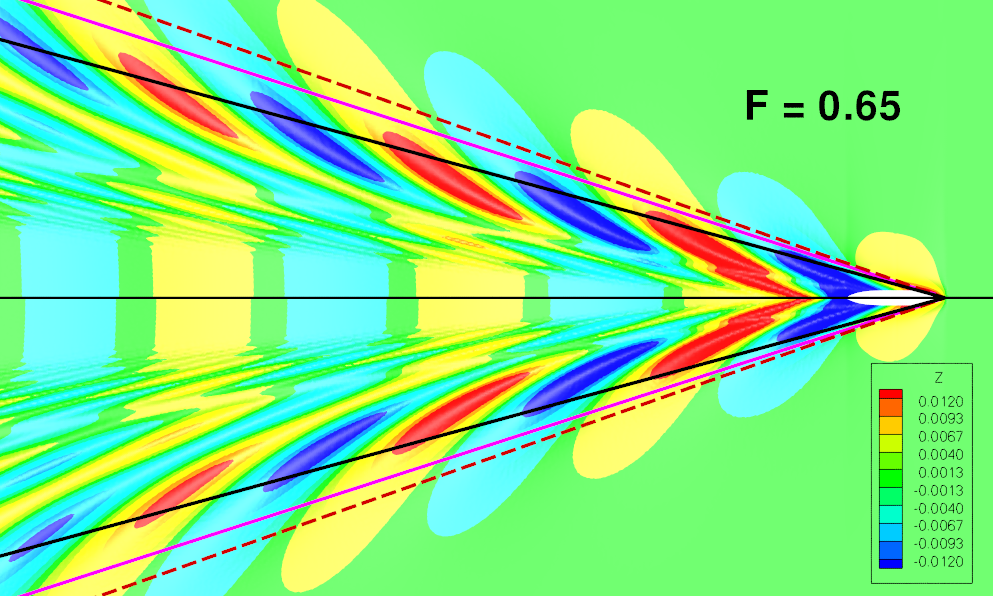
\includegraphics[height=4.3cm]{chap5/065.png}
  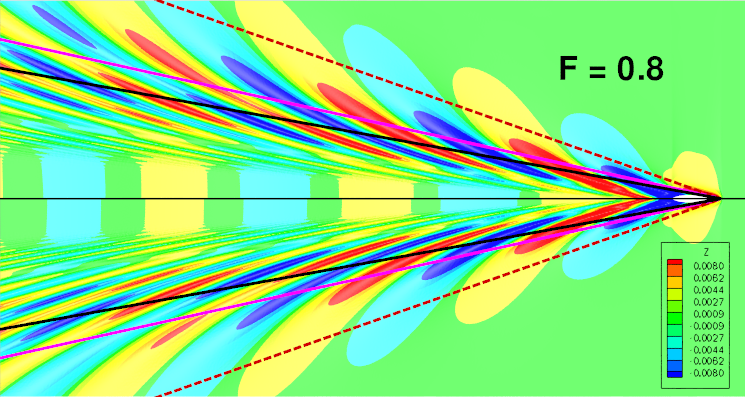
\includegraphics[height=4.3cm]{chap5/08.png}
  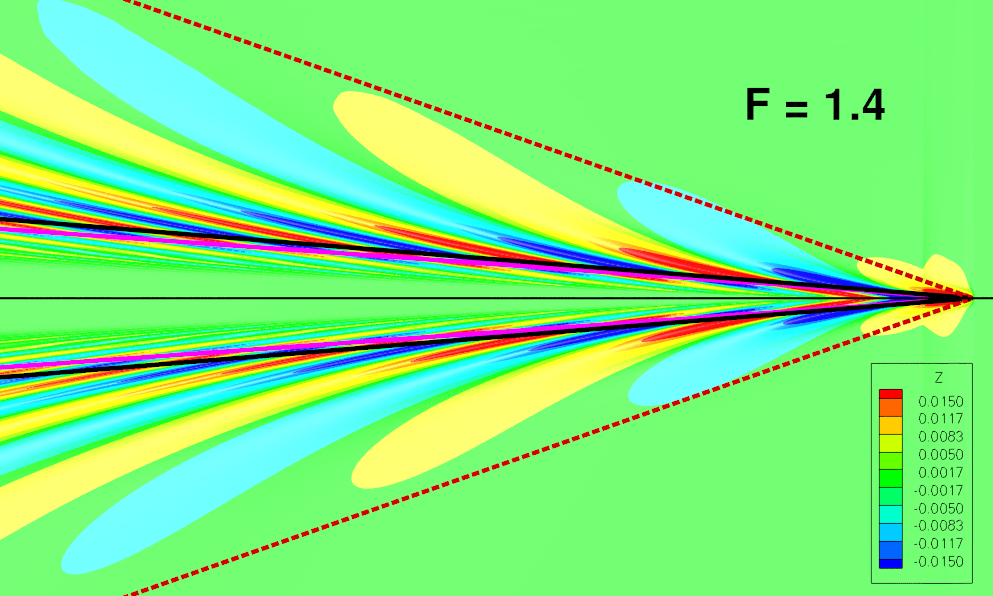
\includegraphics[height=4.3cm]{chap5/14.png}
  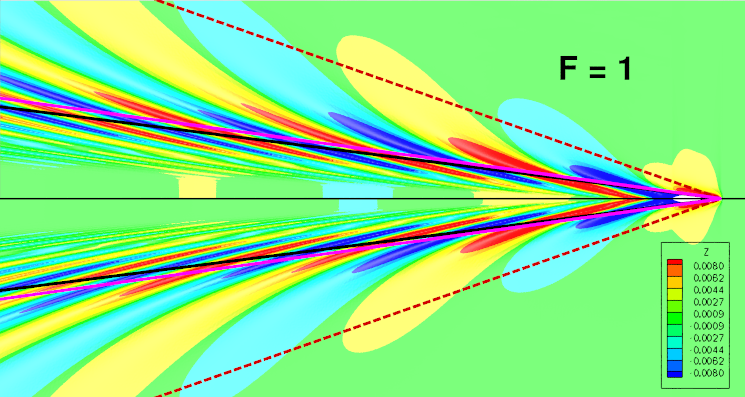
\includegraphics[height=4.3cm]{chap5/10.png}
  \bicaption[fig:wavpatn]{单体船波形图}
  {船体\eqref{eq:simphull}在$F=0.65$、0.8、1和1.4四个Froude数情况下产生的
自由面升高,各波形的上半部分或下半部分由Hogner近似或NM理论计算得出}
{Fig}{Free-surface elevation $Z/L$ for the hull defined by \eqref{eq:simphull} 
at four Froude numbers $F = 0.65$, 0.8, 1 and 1.4. The upper and lower halves 
of the wave patterns are computed via the Hogner approximation or the 
more precise Neumann–Michell theory}
\end{figure}

图\ref{fig:wavpatn}还描画了从船首$(0.5,0)$出发的三种射线。这三种射线分别为
Kelvin臂$\psi=\pm\psi^K\approx19^\circ28'$,
$\psi=\pm\psi^x_{\max}$(黑色实线),由式\eqref{eq:psixmax}定义,
由基于首尾散波系干涉效应的两点兴波模型\supercite{Noblesse2014Why}得出,
以及$\psi=\pm\psi_{\max}$(粉色实线),
由式\eqref{eq:psimaxfit-a}-\eqref{eq:psimaxfit-b}定义,通过数值确定基于Hogner近似
的散波的波幅函数\eqref{eq:zetaD}的第一峰的位置得到。图\ref{fig:wavpatn}表明,
对于$F=1$和$F=1.4$的情况,由高度简化的模型预测的射线$\psi=\pm\psi^x_{\max}$
和这里通过数值方法获得的$\psi=\pm\psi_{\max}$相差不大。
事实上,图\ref{fig:psimaxmonohull}表明当$F\ge1$时两种方法获得的主要兴波角
之间的差异不超过$1^\circ$。然而在$0.6\le F\le1$时,两种方法间差异很大。
图\ref{fig:wavpatn}还表明在$F=0.65$、0.8和1时,由式\eqref{eq:psimaxfit-a}-
\eqref{eq:psimaxfit-b}定义的射线$\psi=\pm\psi_{\max}$位于两点兴波模型得到的
射线$\psi=\pm\psi^x_{\max}$以内,而在$F=1.4$时则相反。

如图\ref{fig:amplfunc}所示,波幅函数\eqref{eq:zetaD}的第一峰在高Froude数
$F\ge0.9$时是尖的,并且显著高于其他峰,但在低Froude数$F=0.7$和$F=0.65$时
是宽的,并且高出其他峰不多。相应地,图\ref{fig:wavpatn}的波形图显示,
在$F=1.4$和$F=1$时,$\psi=\psi_{\max}$附近狭窄的楔状带内波高显著,
而在$F=0.8$和$F=0.65$时,$\psi=\psi_{\max}$附近相对广泛的区域波高显著。
结果意味着,实际观测到船的主要兴波角$\psi_{\max}$在Froude数小于1时
可能比较分散。图\ref{fig:wavpatn}展示的波形与图\ref{fig:amplfunc}展示的
波幅函数\eqref{eq:zetaD}是一致的,正如预期地。

\section{讨论}
\label{sec:discuz}

本章提出了确定任意船体Kelvin波系中波高最大的波浪的射线角与航迹的夹角---主要兴波角
$\psi_{\max}$---的实用方法。该方法只涉及初等运算,可以简单、有效地执行。
具体来说,该方法需要计算由船体表面$\Sigma^H_+$基波\eqref{eq:E}的分布
\eqref{eq:Asymmetry}定义的波幅函数$A$。此方法可以被应用于任意形状的实际船体
(包括多体船)和自由表面压力分布。
因此,该方法比考虑轴对称或椭圆形高斯压力分布更加通用。
此方法密切仿效\parencite{Barnell1986Far},
并且是在船舶水动力学文献中众所周知的基本结论特别是自由表面格林函数的波浪成分
\supercite{Noblesse1981Alternative}
的直接应用。

本章报告的七艘船的计算结果表明单体船的远场波系受分布在船首和船尾区域的
源汇兴波的纵向干涉的显著影响,同时也受到分布于左舷侧和右舷侧区域的源汇兴波的
横向干涉的影响。因此单体船散波间的干涉效应貌似复杂。

两点兴波模型\supercite{Noblesse2014Why}和这里的计算结果表明单体船的兴波特征可以
分为两大区域。当Froude数$F\le F_K$其中$F_K\approx0.6$时,横波系的干涉效应占优势,
因此波高最大的波浪的射线角与航迹的夹角可以用Kelvin角近似,即
$\psi_{\max}\approx\psi^K$。然而在高Froude数$F>F_K$时散波系的干涉效应占优势。
此外,``散波干涉制''$F>F_K$又可细分为三个区域$F_K<F<F_X$,$F_X<F<F_Y$,以及
$F>F_Y$,其中$F_X\apporx0.85$,$F_Y\gg1$。

单体船首尾散波系的纵向干涉在``低速''区域$F_K<F<F_X$占优势,此时主要兴波角
$\psi_{max}$随Froude数以$1/F^2$形式衰减。在``高速''区域$F>F_Y$左右舷侧产生的
散波系的横线干涉占优势,此时$\psi_{\max}$随Froud数按照$1/F$的形式衰减。
这里的计算结果显示,``纵向干涉制''$F_K<F<F_X$和``横向干涉制''$F>F_Y$之间的
过渡是逐步地而非突然地,并且发生在广泛的Froude数区间$F_X<F<F_Y$。

绝大多数排水型船符合``低速横波干涉制''$F\le F_K\approx0.6$或``低速散波干涉制''
$F_K\le F\le F_X\approx0.85$。这两个区域主要受
船体首尾区域产生的横波或散波的纵向干涉效应的影响。这两个区域的实用近似为
\begin{subequations}
\begin{equation}
  \psi_{\max}\approx\psi^K\approx19^\circ28'\quad\text{当}F\le0.573
  \label{eq:transregime}
\end{equation}
和$\tan\psi_{\max}\approx0.16\ell_e/F^2$当$F_K\le F\le F_X$。
图\ref{fig:elleff}展示的实效间距$\ell_e$的数值预测表明,$\ell_e$应该小于
\parencite{Noblesse2014Why}的建议值$\ell_e=0.9$。图\ref{fig:elleff}表明
$\ell_e=0.725$是一个更精确的选择。这个选择给出了以下实用近似
\begin{equation}
  \psi_{\max}\approx\arctan(0.116/F^2)\quad\text{当}0.573\le F\le0.85
  \label{eq:divlongintrfregime}
\end{equation}
在``高速散波干涉制''$F\ge F_X$这里的数值计算给出实用近似
\begin{equation}
  \psi_{\max}\approx\arctan[0.08(1+0.6/F)/F]\quad\text{当}F\ge 0.85
  \label{eq:divlatintrfregime}
\end{equation}
由式\eqref{eq:divlongintrfregime}可知
\begin{equation}
  \psi_{max}\approx\arctan(0.08/F)\quad\text{当}F>6
  \label{eq:veryhigh}
\end{equation}
\end{subequations}
此``超高速''近似与\eqref{eq:psiymax}给出的两点兴波横向干涉结果
$\tan\psi^y_{\max}\approx 0.2\sqrt{b_e}/F$---其中实效型宽$b_e=0.16$---一致。
此区域只出现在超高Froude数情况下,在实际上无法存在,因为$F_Y\approx6$以及超出
线性势流理论的应用范畴。

图\ref{fig:elleff}表明,``纵向干涉关系''$\tan\psi_{\max}\approx0.16\ell_e/F^2$
中实效船首与实效船尾间的实效间距$\ell_e$关于船体形状的变化很大。
然而,图\ref{fig:psimaxmonohull}表明主要兴波角$\psi_{\max}$受船体形状的影响很弱。
事实上,由式\eqref{eq:transregime}-\eqref{eq:divlatintrfregime}给出的实用估计与
主要船体形状参数(长宽比、吃水船长比、宽度吃水比、水线进流角)范围广泛
的七艘船体的数值计算得出的主要兴波角$\psi_{\max}$吻合较好。
此外,即使通过两点兴波模型\supercite{Noblesse2014Why}给出的
基于首尾波系纵向干涉效应的解析近似\eqref{eq:psixmax}也是实际的,尽管
不如式\eqref{eq:transregime}-\eqref{eq:divlatintrfregime}精确,正如我们预期的。
因此表达式\eqref{eq:transregime}-\eqref{eq:divlatintrfregime}提供了估计
一般单体船主要兴波角$\psi_{\max}$的实用估计。

\section{本章小结}

本章考虑在无限深广的静水中匀速直线航行的单体船的窄V字形尾迹。
船体周围的流场以分布在船体表面的点源产生的流场表示,而不是简化为位于船首区域
的一个点源和位于船尾区域的一个点汇。
单体船Kelvin波系中波高最大的波浪所处的射线与航迹的夹角,即主要兴波角
$\psi_{\max}$,通过一种实际的数值方法确定。
这种数值方法只涉及初等运算,因此能够被简单有效地应用。这种方法随后被用于对主尺度
范围广泛的七艘船分别在十个Froude数情况下进行系统的数值计算。
数值研究表明,船体形状的变化对主要兴波角$\psi_{\max}$的影响很弱。
一个有用的实际结果是,一般单体船的主要兴波角$\psi_{\max}$均可通过简单的解析式确定。
这些解析式为主要兴波角$\psi_{\max}(F)$---由式\eqref{eq:transregime}-
\eqref{eq:divlatintrfregime}给出---提供了相对精确的实用估计(无需计算)。
这些主要兴波角$\psi_{\max}(F)$的实用解析式同时考虑了首尾散波系的纵向干涉效应和
由左右舷侧产生的波浪的横向干涉效应。不出所料地,由此得到的主要兴波角的解析式比
两点兴波模型\supercite{Noblesse2014Why}的预测更加精确。
本章提出的主要兴波角$\psi_{\max}$的计算方法可以被轻而易举地应用于双体船。
第\ref{chap:catamaran}章将考虑双体船Kelvin波系中波高最大的波浪的射线角,
即双体船的主要兴波角。



